\documentclass{beamer}
\usepackage[latin1]{inputenc}
\usepackage{comment}
%\usepackage[3D]{movie15}
\usetheme{Warsaw}
\usecolortheme{beaver}
\usefonttheme{structuresmallcapsserif}

\setbeamertemplate{section page}
{
     \tableofcontents[currentsection,hideothersubsections]
}
\setbeamertemplate{subsection page}
{
     \tableofcontents[sectionstyle=show/shaded,subsectionstyle=show/shaded/hide]
}

%\AtBeginSection{\frame{\sectionpage}}
%\AtBeginSubsection{\frame{\subsectionpage}}

\DeclareMathOperator*{\argmin}{arg\,min}
\DeclareMathOperator{\diag}{diag}

\title{Pattern Recognition}
\author{Bertrand Thirion and John Ashburner}
%\institute[j.ashburner@ucl.ac.uk]{Wellcome Trust Centre for Neuroimaging,\\
%UCL Institute of Neurology,\\
%12 Queen Square,\\
%London WC1N 3BG,\\
%UK.}
\date{}
\begin{document}

\begin{frame}
\titlepage
\end{frame}

\section{Introduction}
    \subsection{Definitions}
\begin{frame}
\frametitle{}
\includegraphics[width=\textwidth]{sklearn_material/ml_map.png}
% Note: need some adaptation. Should not be sklearn specific
% useful to clarify the different branches of ML
% 
\end{frame}


\begin{frame}
\frametitle{Some key concepts}

\end{frame}



\begin{comment}
\begin{frame}
\frametitle{General setting}
We have a training dataset of $n$ observations, each consisting of an input ${\bf x}_i$ and a target $y_i$.\par
Each input, ${\bf x}_i$, consists of a vector of $p$ features.
\begin{align*}
\mathcal{D} = \{({\bf x}_i,y_i) | i=1,..,n\}
\end{align*}

The aim is to predict the target for a new input ${\bf x}_*$.
\end{frame}

\begin{frame}
\frametitle{Classification}
\begin{columns}
\column{0.4\textwidth}
Targets (${\bf y}$) are categorical labels.\par
Train with $\mathcal{D} = \{({\bf x}_i,y_i) | i=1,..,n\}$ and use result to make best guess of $y_*$ given ${\bf x}_*$.
\column{0.6\textwidth}
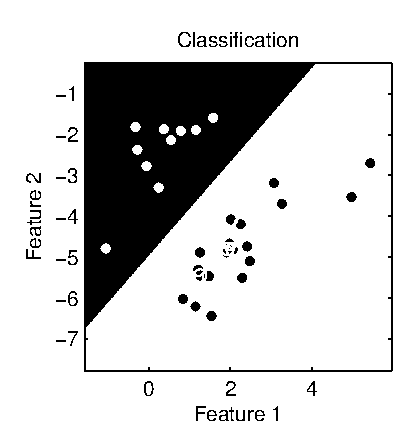
\includegraphics[width=\textwidth]{simple_classification}
\end{columns}
\end{frame}

\begin{frame}
\frametitle{Probabilistic classification}
\begin{columns}
\column{0.4\textwidth}
Targets (${\bf y}$) are categorical labels.\par
Train with $\mathcal{D} = \{({\bf x}_i,y_i) | i=1,..,n\}$ and compute $P(y_*=1 | {\bf x}_*, \mathcal{D})$.
\column{0.6\textwidth}
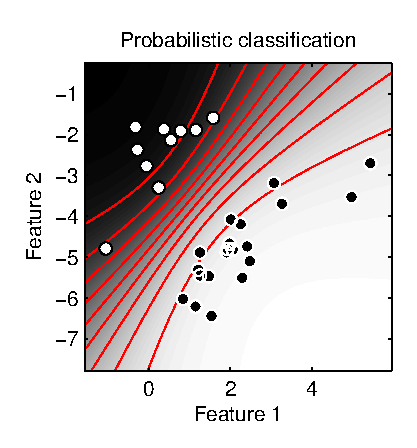
\includegraphics[width=\textwidth]{probabilistic_classification}
\end{columns}
\end{frame}

\begin{frame}
\frametitle{Regression}
\begin{columns}
\column{0.4\textwidth}
Targets (${\bf y}$) are continuous real variables.\par
Train with $\mathcal{D} = \{({\bf x}_i,y_i) | i=1,..,n\}$ and compute $p(y_* | {\bf x}_*, \mathcal{D})$.
\column{0.6\textwidth}
\includegraphics[width=\textwidth]{regression}
\end{columns}
\end{frame}

\begin{frame}
\frametitle{Many other settings}
\begin{itemize}
\item {\bf Multi-class classification} when there are more than two possible categories.
\item {\bf Ordinal regression} for classification when there is some ordering of the categories.\par
\begin{tiny}
Chu, Wei, and Zoubin Ghahramani. ``Gaussian processes for ordinal regression.'' In Journal of Machine Learning Research, pp. 1019-1041. 2005.\par
\end{tiny}
\item {\bf Multi-task learning} when there are multiple targets to predict, which may be related.
\item etc
\end{itemize}
\end{frame}
\end{comment}

    \subsection{Classification and Regression}                               \begin{frame}
\frametitle{General setting}
We have a training dataset of $n$ observations, each consisting of an input ${\bf x}_i$ and a target $y_i$.\par
Each input, ${\bf x}_i$, consists of a vector of $p$ features.
\begin{align*}
\mathcal{D} = \{({\bf x}_i,y_i) | i=1,..,n\}
\end{align*}

The aim is to predict the target for a new input ${\bf x}_*$.
\end{frame}


    \subsection{Curse of Dimensionality}                                     \begin{frame}
\frametitle{Curse of dimensionality}
\begin{center}
{\Huge Large $p$, small $n$.\par}
\end{center}
\end{frame}

\begin{frame}
\frametitle{Nearest-neighbour classification}
\begin{columns}[c]
\column{0.7\textwidth}
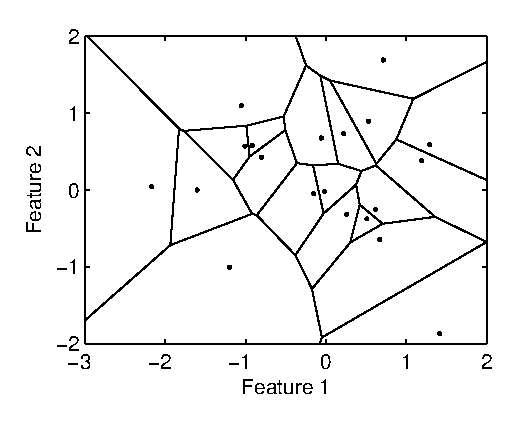
\includegraphics[width=\textwidth]{voronoi}
\column{0.3\textwidth}
\begin{itemize}
\item Not nice smooth separations.
\item Lots of sharp corners.
\item May be improved with \emph{K-nearest neighbours}.
\end{itemize}
\end{columns}
\end{frame}

\begin{frame}
\frametitle{Rule-based approaches}
\begin{columns}[c]
\column{0.7\textwidth}
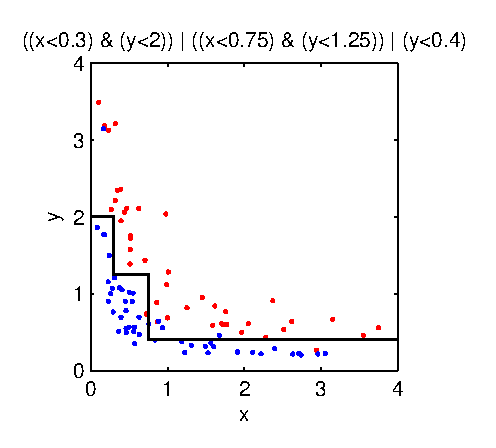
\includegraphics[width=\textwidth]{rule_based}
\column{0.3\textwidth}
\begin{itemize}
\item Not nice smooth separations.
\item Lots of sharp corners.
\end{itemize}
\end{columns}
\end{frame}


\begin{frame}
\frametitle{Corners matter in high-dimensions}
\begin{columns}[c]
\column{0.4\textwidth}
\includegraphics[width=\textwidth]{circle}
\column{0.6\textwidth}
\includegraphics[width=\textwidth]{sphere}
\end{columns}
\end{frame}

\begin{frame}
\frametitle{Corners matter in high-dimensions}
\begin{columns}[c]
\column{0.2\textwidth}
\includegraphics[width=.8\textwidth]{circle}

\includegraphics[width=\textwidth]{sphere}
\column{0.8\textwidth}
\includegraphics[width=\textwidth]{corners}
\end{columns}
\end{frame}

\begin{frame}
\frametitle{Dimensionality $\ne$ number of voxels}
\begin{itemize}
\item Little evidence to suggest that most voxel-based feature selection methods help.
\begin{itemize}
\item Little or no increase in predictive accuracy.
\item Commonly perceived as being more ``interpretable''.
\end{itemize}
\item Prior knowledge derived from independent data is the most reliable way to improve accuracy.
\begin{itemize}
\item e.g. search the literature for clues about which regions to weight more heavily.
\end{itemize}
\end{itemize}

\vspace{1cm}
{\tiny Cuingnet, R\'emi, Emilie Gerardin, J\'er\^ome Tessieras, Guillaume Auzias, St\'ephane Leh\'ericy, Marie-Odile Habert, Marie Chupin, Habib Benali, and Olivier Colliot. ``Automatic classification of patients with Alzheimer's disease from structural MRI: a comparison of ten methods using the ADNI database.'' Neuroimage 56, no. 2 (2011): 766-781.\par}
{\tiny Chu, Carlton, Ai-Ling Hsu, Kun-Hsien Chou, Peter Bandettini, and ChingPo Lin. ``Does feature selection improve classification accuracy? Impact of sample size and feature selection on classification using anatomical magnetic resonance images.'' Neuroimage 60, no. 1 (2012): 59-70.\par}
{\tiny See winning strategies in \url{http://www.ebc.pitt.edu/PBAIC.html}\par}
\end{frame}

\begin{frame}
\frametitle{Linear versus Nonlinear methods}
\begin{columns}[c]
\column{0.7\textwidth}
\begin{itemize}
\item Linear methods are more interpretable.
\item Nonlinear methods usually increase dimensionality.
\item Better to preprocess to obtain features that behave more linearly.
\end{itemize}
\includegraphics[width=\textwidth]{bmi}
\column{0.3\textwidth}
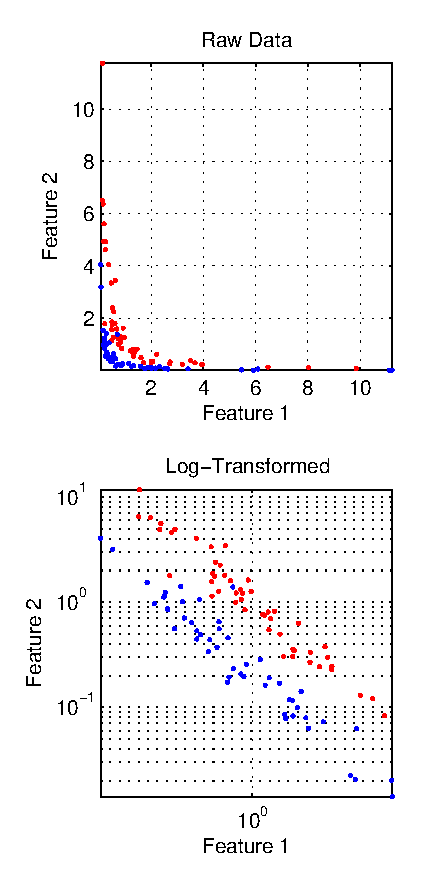
\includegraphics[width=\textwidth]{log_transformed}
\end{columns}
\end{frame}


\section{Generalization of learned models across datasets}
    \subsection{Cross-Validation}                                            
\begin{frame}
\frametitle{Occam's razor}
\begin{quote}
``Everything should be kept as simple as possible, but no simpler.''
\par \rightline{\tiny{\rm --- Einstein (allegedly)}}
\end{quote}
\vspace{0.25cm}
\begin{itemize}
\item Complex models (with many estimated parameters) usually explain training data better than simpler models.\par
\item Simpler models often generalise better to new data than more complex models.\par
\end{itemize}
Need to find the model with the optimal bias/variance tradeoff.\par
\end{frame}

\begin{frame}
\frametitle{Bayesian model selection}
\emph{Real Bayesians don't cross-validate} (except when they need to).\par
\begin{align*}
P(M|\mathcal{D}) = \frac{p(\mathcal{D}|M) P(M)}{p(\mathcal{D})}\\
\end{align*}
The \emph{Bayes factor} allows the plausibility of two models ($M_1$ and $M_2$) to be compared:
\begin{align*}
K = \frac{p(\mathcal{D}|M_1)}{p(\mathcal{D}|M_2)} =
    \frac{\int_{\theta_{M_1}} p(\mathcal{D}|\theta_{M_1},M_1) p(\theta_{M_1}|M_1) d{\theta}_{M_1}}
         {\int_{\theta_{M_2}} p(\mathcal{D}|\theta_{M_2},M_2) p(\theta_{M_2}|M_2) d{\theta}_{M_2}}
\end{align*}
This is usually too costly in practice, so approximations are used.
\end{frame}

\begin{frame}
\frametitle{Model selection}
%\begin{quote}``In theory there is no difference between theory and practice. In practice there is.''
%\par \rightline{\tiny{\rm --- Yogi Berra}}
%\end{quote}
Some approximations/alternatives to the Bayesian approach:
\begin{itemize}
\item {\bf Laplace approximations}: find the MAP/ML solution and use a Gaussian approximation to the parameter uncertainty.
\item {\bf Minimum Message Length} (MML): an information theoretic approach.
\item {\bf Minimum Description Length} (MDL): an information theoretic approach based on how well the model compresses the data.
\item {\bf Akaike Information Criterion} (AIC): $-2\log p(\mathcal{D}|\theta) + 2 k$, where $k$ is the number of estimated parameters.
\item {\bf Bayesian Information Criterion} (BIC): $-2\log p(\mathcal{D}|\theta) + k\log q$, where $q$ is the number of observations.
%\item {\bf Deviance Information Criterion} (DIC) and others.
\end{itemize}
\end{frame}

\begin{frame}
\frametitle{Model selection by nested cross-validation}

Inner cross-validation loop used to evaluate model's performance on a
pre-defined grid of parameters and retain the best one.

\begin{itemize}
\item Safe, but costly.
\item Supported by some libraries (e.g. scikit-learn).
\includegraphics[width=\textwidth]{sklearn_material/grid}\\
\includegraphics[width=.65\textwidth]{sklearn_material/grid_search}
\item Some estimators have path model, hence allow faster evaluation
  (e.g. LASSO).
\item Randomized techniques also exist, sometimes more efficient.
\item \textbf{Caveat:} Inner cross-validation loop $\neq$ outer
  cross-validation loop for parameter evaluation.
\end{itemize}
\end{frame}

\begin{frame}
\frametitle{Parameter setting and overfit} 

Using one cross-validation loop for learning parameters and evaluating
yields \textbf{optimistic bias} and \textbf{poor generalization}:
Overfit ! {\tiny \url{http://nilearn.github.io/building_blocks/estimator_choice.html}}

\includegraphics[width=.8\textwidth]{sklearn_material/plot_haxby_grid_search_11.png}

\end{frame}

    \subsection{Accuracy Measures}                                           
\begin{frame}
\frametitle{Accuracy measures for regression}
\begin{itemize}
\item {\bf Root-mean squared error} for point predictions.
\item {\bf Correlation coefficient} for point predictions.
\item {\bf Log predictive probability} can be used for probabilistic predictions.
\item {\bf Expected loss/risk} for point predictions for decision making.
\end{itemize}
\end{frame}

\begin{frame}
\frametitle{Accuracy measures for binary classification}
\begin{columns}
\column{0.7\textwidth}
\includegraphics[width=\textwidth]{contingency_table_wikipedia}
%\vspace{0.25cm}
\column{0.3\textwidth}
%\includegraphics[width=\textwidth]{spec_sens_wikipedia}
\begin{tiny}
Wikipedia contributors, ``Sensitivity and specificity,'' Wikipedia, The Free Encyclopedia, \url{http://en.wikipedia.org/w/index.php?title=Sensitivity\_and\_specificity\&oldid=655245669} (accessed April 9, 2015).\par
\end{tiny}
\end{columns}
\end{frame}

\begin{frame}
\frametitle{Accuracy measures from ROC curve}
\begin{columns}
\column{0.5\textwidth}
The {\bf Receiver operating characteristic} (ROC) curve is a plot of \emph{true-positive rate} (sensitivity) versus \emph{false-positive rate} (1-specificity) over the full range of possible thresholds.\par
\vspace{0.25cm}
The {\bf area under the curve} (AUC) is the integral under the ROC curve.\par
\column{0.5\textwidth}
\includegraphics[width=\textwidth]{roc}
\end{columns}
\end{frame}

\begin{frame}
\frametitle{Log predictive probability}
Some data are more easily classified than others.\par
Probabilistic classifiers provide a level of confidence for each prediction.
\begin{align*}
p(y_*|{\bf x}_*,{\bf y},{\bf X},\theta)
\end{align*}
Quality of predictions can be assessed using the {\bf test log predictive probability}:
\begin{align*}
\tfrac{1}{m}\sum_{i=1}^m \log_2 p(y_{*i}\!=\!t_i|{\bf x}_{*i},{\bf y},{\bf X},\theta)
\end{align*}
After subtracting the baseline measure, this shows the average bits of information given by the model.\par
\vspace{0.25cm}
\begin{tiny}
Rasmussen \& Williams. ``Gaussian Processes for Machine Learning'', MIT Press (2006).\par
\url{http://www.gaussianprocess.org/gpml/}\par
\end{tiny}
\end{frame}


    \subsection{Parameter Tuning}                                            \include{ParameterTuning}
\section{Overview of the main methods}

\begin{frame}
\frametitle{Overview of classification tools}
\hspace*{-1cm}
\includegraphics[width=1.2\textwidth]{sklearn_material/plot_classifier_comparison_001.png}\\
Only one rule: No tool wins in all situations. 
\end{frame}



    \subsection{Simple Generative Models: Naive Bayes, Linear Discriminant Analysis}       
\begin{frame}
\frametitle{Generative models for classification}
\begin{columns}[c]
\column{0.5\textwidth}
\begin{align*}
P(y\!=\!k|{\bf x}) = \frac{P(y\!=\!k) p({\bf x}|y\!=\!k)}{\sum_j P(y\!=\!j) p({\bf x}|y\!=\!j)}
\end{align*}
\column{0.5\textwidth}
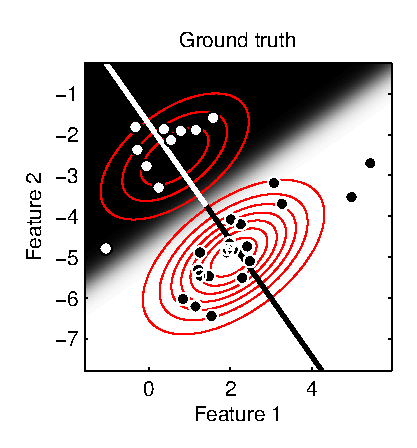
\includegraphics[width=\textwidth]{simple_ground_truth}
\end{columns}
\end{frame}

\begin{frame}
\frametitle{Linear discriminant analysis}
\begin{columns}[c]
\column{0.5\textwidth}
\begin{align*}
P(y\!=\!k|{\bf x}) = \frac{P(y\!=\!k) p({\bf x}|y\!=\!k)}{\sum_j P(y\!=\!j) p({\bf x}|y\!=\!j)}
\end{align*}
Assumes:
\begin{align*}
P({\bf x}|y\!=\!k) = \mathcal{N}({\bf x} | {\boldsymbol\mu}_k, \boldsymbol\Sigma)
\end{align*}
\column{0.5\textwidth}
\includegraphics[width=\textwidth]{simple_fld}
\end{columns}
Model has $2p + p(p-1)$ parameters to estimate (two means and a single covariance).\par
Number of observations is $pn$ (size of inputs).
\end{frame}

\begin{frame}
\frametitle{Quadratic discriminant analysis}
\begin{columns}[c]
\column{0.5\textwidth}
\begin{align*}
P(y\!=\!k|{\bf x}) = \frac{P(y\!=\!k) p({\bf x}|y\!=\!k)}{\sum_j P(y\!=\!j) p({\bf x}|y\!=\!j)}
\end{align*}
Assumes different covariances:
\begin{align*}
P({\bf x}|y\!=\!k) = \mathcal{N}({\bf x} | {\boldsymbol\mu}_k, {\boldsymbol\Sigma}_k)
\end{align*}
\column{0.5\textwidth}
\includegraphics[width=\textwidth]{simple_qda}
\end{columns}
Model has $2p + 2p(p-1)$ parameters to estimate (two means and two covariances).\par
Number of observations is $pn$.
\end{frame}

\begin{frame}
\frametitle{Naive Bayes}
\begin{columns}[c]
\column{0.5\textwidth}
\begin{align*}
P(y\!=\!k|{\bf x}) = \frac{P(y\!=\!k) p({\bf x}|y\!=\!k)}{\sum_j P(y\!=\!j) p({\bf x}|y\!=\!j)}\cr
\end{align*}
Assumes that features are independent:
\begin{align*}
p({\bf x}|y\!=\!k) = \prod_i p(x_i|y\!=\!k)
\end{align*}
\column{0.5\textwidth}
\includegraphics[width=\textwidth]{simple_naive_bayes}
\end{columns}
Model has variable number of parameters to estimate, but the above example has $3p$.\par
Number of observations is $pn$.
\end{frame}


    \subsection{Simple Discriminative Models: Gaussian Processes, Support-Vector Machines} \begin{frame}
\frametitle{There is more than just classification}
\begin{columns}[c]
\column{.4\textwidth}
\begin{itemize}
\item Canonical Correlation Analysis
\item Multi-Way, Multi-View Learning
\item Other existing methods
\item Methods not yet invented
\end{itemize}
\column{.6\textwidth}
\includegraphics[width=\textwidth]{huopaniemi}

{\itshape\tiny Huopaniemi, Ilkka, Tommi Suvitaival, Janne Nikkil\"{a}, Matej Ore\v{s}i\v{c}, and Samuel Kaski. ``Multi-way, multi-view learning.'' arXiv preprint arXiv:0912.3211 (2009).\par}
\end{columns}
\end{frame}


\begin{frame}
\frametitle{Kernel Matrices}
Linear kernel matrices may computed from the raw features.
\begin{eqnarray*}
{\bf C} = {\bf V}{\bf V}^T
\end{eqnarray*}
A simple spatial feature selection may be considered as the following, where ${\bf A}$ is a diagonal matrix of ones and zeros:
\begin{eqnarray*}
{\bf C} = {\bf V}{\bf A}{\bf V}^T
\end{eqnarray*}
However, ${\bf A}$ may be more complicated, for example encoding spatial smoothing, high-pass filtering or any number of other things.
\end{frame}

\begin{frame}
\frametitle{Inner Products}
This gives us an alternative way of measuring distances between vectors in a linear way, where ${\bf A}$ is symmetric and positive definite.
\begin{eqnarray*}
d({\bf v}_1,{\bf v}_2) = \sqrt{({\bf v}_1 - {\bf v}_2)^T {\bf A} ({\bf v}_1 - {\bf v}_2)}
\end{eqnarray*}

Usually, the operation ${\bf A}{\bf v}^T$ is performed as a convolution.  For example, when dealing with 2D data, we may convolve with the Laplacian operator.
\begin{eqnarray*}
{\nabla}^2 {\bf v} = {\bf v} \ast \begin{pmatrix} 0 & -1 & 0\cr -1 & 4 & -1\cr 0 & -1 & 0\end{pmatrix}
\end{eqnarray*}

Note that the actual form of ${\bf A}$ can vary, so we need to figure out what metric tensor is optimal.
\end{frame}


    \subsection{Basic Regularization Methods}                                \include{BasicRegularisationMethods}
\section{Model Averaging}
    \subsection{Boosting \& Bagging}                                         \begin{frame}
\frametitle{Ensemble learning}
Combining predictions from weak learners.
\begin{itemize}
\item {\bf Bootstrap aggregating (bagging)}
\begin{itemize}
\item Train several weak classifiers, with different models or randomly drawn subsets of the data.
\item Average their predictions with equal weight.
\end{itemize}
\item {\bf Boosting}
\begin{itemize}
\item A family of approaches, where models are weighted according to their accuracy.
\item AdaBoost is popular, but has problems with target noise.
\end{itemize}
\item {\bf Bayesian model averaging}
\begin{itemize}
\item Really a model selection method.
\item Relatively ineffective for combining models.
\end{itemize}
\item {\bf Bayesian model combination}
\begin{itemize}
\item Shows promise.
\end{itemize}
\end{itemize}
\begin{tiny}
Monteith, et al. ``Turning Bayesian model averaging into Bayesian model combination.'' Neural Networks (IJCNN), The 2011 International Joint Conference on. IEEE, 2011.\par
\end{tiny}
\end{frame}

\begin{frame}
\frametitle{Random Forests}
\end{frame}


    \subsection{Decision trees and Random Forests}                           \include{RandomForests}
\section{Resources}                                                          \begin{frame}
\frametitle{Free Books}
\begin{itemize}
\item {\bf The Elements of Statistical Learning: Data Mining, Inference, and Prediction}
      Trevor Hastie, Robert Tibshirani, Jerome Fried(2009)
      \url{http://statweb.stanford.edu/~tibs/ElemStatLearn/}
\item {\bf An Introduction to Statistical Learning with Applications in R}
      Gareth James, Daniela Witten, Trevor Hastie and Robert Tibshirani (2013)
      \url{http://www-bcf.usc.edu/\%7Egareth/ISL/}
\item {\bf Introduction to Machine Learning}
      Amnon Shashua (2008)
      \url{http://arxiv.org/pdf/0904.3664.pdf}
\end{itemize}
\end{frame}

\begin{frame}
\frametitle{Free Books}
\begin{itemize}
\item {\bf Bayesian Reasoning and Machine Learning}
      David Barber (2014)
      \url{http://www.cs.ucl.ac.uk/staff/d.barber/brml/}
\item {\bf Gaussian Processes for Machine Learning}
      Carl Edward Rasmussen and Christopher K. I. Williams (2006)
      \url{http://www.gaussianprocess.org/gpml/chapters/}
\item {\bf Information Theory, Inference, and Learning Algorithms}
      David J.C. MacKay (2003)
      \url{http://www.inference.phy.cam.ac.uk/itila/book.html}
\end{itemize}
\end{frame}

\begin{frame}
\frametitle{Web sites}
\begin{itemize}
\item {\bf Kernel Machines} \url{http://www.kernel-machines.org/}
\item {\bf The Gaussian Processes Web Site} includes links to software. \url{http://www.gaussianprocess.org/}
\item {\bf SVM - Support Vector Machines} includes links to software. \url{http://www.support-vector-machines.org/}
\item {\bf Pascal Video Lectures}  \url{http://videolectures.net/pascal}
\end{itemize}
\end{frame}

\begin{frame}
\frametitle{MATLAB tools}
\begin{itemize}
\item \textbf{Spider} Object orientated environment for machine learning in MATLAB.
\item \textbf{GPML} Gaussian processes for supervised learning. % (\url{http://www.gaussianprocess.org/gpml/code/matlab/doc/}).
\item \textbf{Pronto} MATLAB ML tbx for neuroimaging. GUI. Implements many ML concepts. Continuity with SPM.
\end{itemize}
\end{frame}

\begin{frame}
\frametitle{Python tools}
\begin{itemize}
\item \textbf{Scikit-learn} Generic ML in Python. Complete,
  high-quality, well-documented, reference implementations.
\item \textbf{Nilearn} Python interface to Scikit-learn for
  Neuroimaging. Easy-to-use/install. Good viz.
\item \textbf{Pymvpa} Python tool for ML. Advanced stuff
  (Pipelines, Hyperalignment).
\end{itemize}
\end{frame}


\end{document}

